\documentclass[12pt]{article}
\usepackage[utf8]{inputenc}
\usepackage{amssymb, amsmath,graphicx,hyperref,xcolor}

\setlength{\parindent}{0in}
\setlength{\parskip}{1em}

\usepackage{fancyhdr}
\rhead{}

\pagestyle{fancy}
\lhead{St Olaf College}
\chead{CS 241}
\rhead{Spring 2024}

\cfoot{\thepage}

\begin{document}

Name: \makebox[3in]{\hrulefill
%NAME
\hrulefill}

\vfill

\begin{center}
{\huge Final Exam}
\end{center}

\begin{itemize}

    \item This exam covers the following standards: %STANDARDS
    .
    \item Please use as much scratch paper as you need to ensure that your answers are complete and legible.
    \item I have confidence in you!
\end{itemize}

\vfill

I pledge my honor that on this examination I have neither given nor received assistance not explicitly approved by the professor and that I have seen no dishonest work 

\hfill Signed: \makebox[3in]{\hrulefill}

$\square$\quad I have intentionally not signed the pledge. (check only if appropriate)
\newpage

%BEGIN_DR

\section*{Data Representation}

\begin{enumerate}
\item Convert the unsigned binary number \texttt{0b00100001} to decimal.
\vfill

\item Convert the decimal integer \texttt{-23} to 8-bit two's complement binary.
\vfill

\item Compute the following subtraction of two's complement binary integers: \texttt{0b00111000 - 0b00010111}. Leave your answer in binary.
\vfill

\item Convert the hexadecimal number \texttt{0x05FE} directly to unsigned binary.
\vfill

\item Write the string \texttt{"Hello!"} as a sequence of ASCII values. An ASCII table is included on the next page.
\vfill
\end{enumerate}

\vfill

\rule[1ex]{\textwidth}{.1pt}

$\square$ \textbf{P}: You have demonstrated proficiency. Full credit. Well done!

$\square$ \textbf{S}: Partial proficiency. Half credit

$\square$ \textbf{I}: You have not yet demonstrated proficiency

\newpage

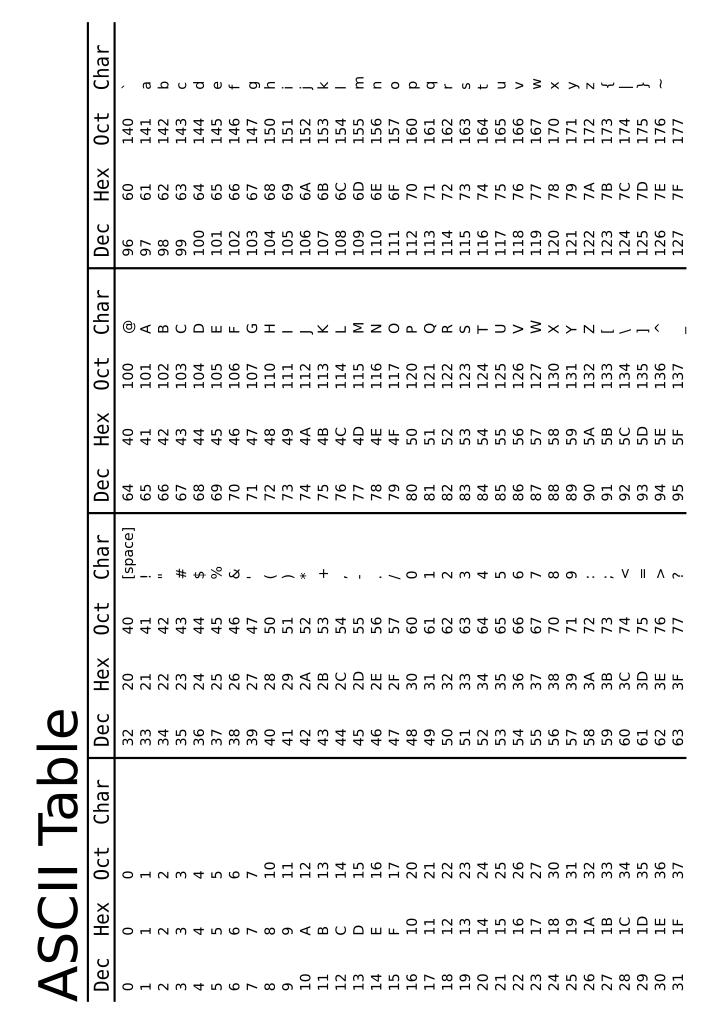
\includegraphics[width=\textwidth]{wikimedia-ascii-table.png}

\newpage

%END_DR

%BEGIN_LR

\section*{Logic Representation}

\begin{enumerate}
\item Consider the boolean function \texttt{f(A,B,C)=(A NAND B) XOR (NOT C)}. Make a truth table for this function. Draw a logic circuit for this function.

\vfill

\item Let \texttt{f(A, B, C)} be true if \texttt{A}, \texttt{B}, and \texttt{C} are all true, false otherwise. Write \texttt{f} in terms of the basic boolean functions \texttt{AND}, \texttt{OR}, \texttt{NOT}, \texttt{NAND}, \texttt{NOR}, and/or \texttt{XOR}. 
\vfill

\item Draw a logic circuit representing the sum of two one-bit unsigned binary numbers: \texttt{0bA + 0bB = 0bCD}. There should be two input bits (\texttt{A} and \texttt{B}) and two output bits (\texttt{C} and \texttt{D}). 
\vfill
\end{enumerate}

\vfill

\rule[1ex]{\textwidth}{.1pt}

$\square$ \textbf{P}: You have demonstrated proficiency. Full credit. Well done!

$\square$ \textbf{S}: Partial proficiency. Half credit

$\square$ \textbf{I}: You have not yet demonstrated proficiency

\newpage

%END_LR

%BEGIN_HC

\section*{Hardware Components}

\begin{enumerate}
\item What is the role of main memory in a computer?
\vfill

\item What is the role of the control unit in a computer?
\vfill

\item What is the role of the central processing unit in a computer?
\vfill

\item What is the role of the arithmetic logic unit in a computer?
\vfill

\item What are cores, processes, and threads? How do they relate, and how are they different?
\vfill

\item Your Raspberry Pi has a 64-bit CPU with a clock speed of 1.5GHz. What do these numbers mean?
\end{enumerate}

\vfill

\rule[1ex]{\textwidth}{.1pt}

$\square$ \textbf{P}: You have demonstrated proficiency. Full credit. Well done!

$\square$ \textbf{S}: Partial proficiency. Half credit

$\square$ \textbf{I}: You have not yet demonstrated proficiency

\newpage

%END_HC

%BEGIN_HI

\section*{Hardware Interactions}


\begin{enumerate}
\item Write a detailed explanation of what happens in the fetch phase. Be sure to include which hardware components are involved, how each hardware component is involved, and what information is sent over the control, data, and address bus.
\vfill

\item Same as above, but for the decode phase.
\vfill

\item Same as above, but for the execute phase.
\vfill

\item Same as above, but for the store phase.
\vfill

\item Explain how CPU pipelining works.
\vfill

\item What is a data hazard?
\vfill

\item What is a control hazard?
\end{enumerate}

\vfill

\rule[1ex]{\textwidth}{.1pt}

$\square$ \textbf{P}: You have demonstrated proficiency. Full credit. Well done!

$\square$ \textbf{S}: Partial proficiency. Half credit

$\square$ \textbf{I}: You have not yet demonstrated proficiency

\newpage

%END_HI

%BEGIN_MD

\section*{Memory Diagrams}

The following page has an Assembly program. It does the following:
\begin{itemize}
    \item Allocate a local variable \texttt{x} and store a value to it
    \item Call the function \texttt{get\_square} on \texttt{x}
    \item Back in main, print the results
\end{itemize}

The output looks like:
\begin{verbatim}
    16 squared is 256
\end{verbatim}

Please draw \underline{two memory diagrams}, one for each of the indicated lines. The diagram should show the values in registers and main memory at that time. In cases where you don't know the literal value, write what it is --- for example, ``old lr". 


\vfill

\rule[1ex]{\textwidth}{.1pt}

$\square$ \textbf{P}: You have demonstrated proficiency. Full credit. Well done!

$\square$ \textbf{S}: Partial proficiency. Half credit

$\square$ \textbf{I}: You have not yet demonstrated proficiency

\newpage

\begin{verbatim}
    .section .rodata
output: .ascii "%d squared is %d\n\0"

    .text
get_square:
    push {fp, lr}
    add fp, sp, #4
    ldr r3, [r0]
    @ square it and store the result
    mul r3, r0, r0
    mov r0, r3
    @             STOP HERE FOR MEMORY DIAGRAM 1
    pop {fp, pc}

    .global main
main: 
    push {fp, lr}
    add fp, sp, #4
    sub sp, sp, #4
    @ fp-8 is x
    mov r1, #16
    str r1, [fp, #-8]
    @ load x and pass it into the function
    ldr r0, [fp, #-8]
    bl square_by_address
    @ print the results
    mov r2, r0
    ldr r1, [fp, #-8]
    @             STOP HERE FOR MEMORY DIAGRAM 2
    ldr r0, output_ptr
    bl printf
    mov r0, #0
    sub sp, fp, #4
    pop {fp, pc}

output_ptr: .word output
\end{verbatim}

%END_MD

%BEGIN_AP1

\section*{Assembly Programming I}

The following page has the skeleton of an Assembly program with comments. The program does the following:
\begin{itemize}
    \item Create global variables \texttt{n\_sandwiches} and \texttt{n\_slices}
    \item Use \texttt{printf} to ask the user how many sandwiches they have
    \item Use \texttt{scanf} to accept a value and store it to \texttt{n\_sandwiches}
    \item Multiply the value by two and store it in \texttt{n\_slices}
    \item Use \texttt{printf} to report the number of slices of bread
\end{itemize}

For example:
\begin{verbatim}
    How many sandwiches do you have? 4
    That's 8 slices of bread!
\end{verbatim}

Please fill in the missing code

\vfill

\rule[1ex]{\textwidth}{.1pt}

$\square$ \textbf{P}: You have demonstrated proficiency. Full credit. Well done!

$\square$ \textbf{S}: Partial proficiency. Half credit

$\square$ \textbf{I}: You have not yet demonstrated proficiency

\newpage

\begin{verbatim}
@ global constants



@ global variables



@ main


    
    @ stack frame setup, no local variables



    @ print the prompt



    @ read the value n_sandwiches



    @ compute n_slices and store the value



    @ load n_slices and print the reply



    @ stack frame teardown, return zero



@ pointers
\end{verbatim}

%END_AP1

%BEGIN_AP2

\section*{Assembly Programming II}

The following page has the skeleton of an Assembly program with comments. The program does the following:
\begin{itemize}
    \item Allocate local variables \texttt{x} and \texttt{x\_plus\_two} in \texttt{main}
    \item Store the value \texttt{12} in \texttt{x}
    \item Call the function \texttt{add\_one} with input \texttt{x}
    \item Call the function \texttt{add\_one} again on the return value from the first call
    \item Store the final result in \texttt{x\_plus\_two}
\end{itemize}

Please fill in the missing code

\vfill

\rule[1ex]{\textwidth}{.1pt}

$\square$ \textbf{P}: You have demonstrated proficiency. Full credit. Well done!

$\square$ \textbf{S}: Partial proficiency. Half credit

$\square$ \textbf{I}: You have not yet demonstrated proficiency

\newpage

\begin{verbatim}
@ function add_one



    @ return input + 1



@ function main


    
    @ stack frame setup, two local variables



    @ store initial value for x



    @ call add_one



    @ call add_one again



    @ store x_plus_two



    @ stack frame teardown, return 0



\end{verbatim}

%END_AP2

%BEGIN_AP3

\section*{Standard: Assembly Programming III}

The following page has the skeleton of an Assembly program that uses a loop to add up the numbers from 1 to 1000. Please fill in the missing code. 

Note: there are a few different ways to write a loop. Your code does not need to line up exactly with the comments.

Also note: there is a formula to compute this sum directly. Do not use the formula. Use a loop.

\vfill

\rule[1ex]{\textwidth}{.1pt}

$\square$ \textbf{P}: You have demonstrated proficiency. Full credit. Well done!

$\square$ \textbf{S}: Partial proficiency. Half credit

$\square$ \textbf{I}: You have not yet demonstrated proficiency

\newpage

\begin{verbatim}
    .section .rodata
result: .ascii "The sum from 0 to 1000 is: %d\n\0"

    .text
    .global main
main: 
    @ stack frame setup, no local variables
    push {fp, lr}
    add fp, sp, #4
    @ initialize loop counter and sum




    @ increment loop counter



    
    @ update the sum


    
    
    @ check loop condition, maybe repeat



    
    @ report result
    ldr r0, result_ptr
    mov r1, r5
    bl printf
    @ return 0, stack frame teardown
    mov r0, #0
    pop {fp, pc}

result_ptr: .word result
\end{verbatim}

%END_AP3

\end{document}
